\section{Projects}
\label{sec:}

In this section we present a sampling of projects that 
illustrate the capabilities of the micro:bit. 

\begin{figure} 
    \begin{tabular}{cc}
        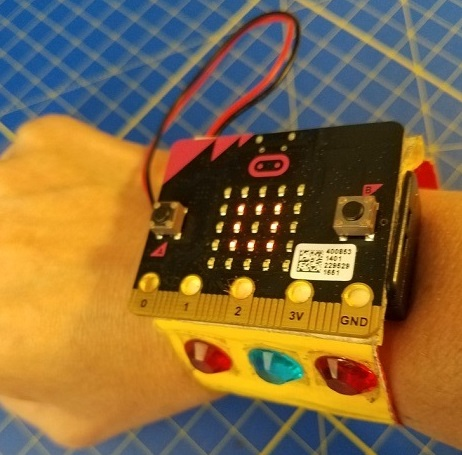
\includegraphics[width=1.5in]{images/rock-paper-scissors.jpg}  &
        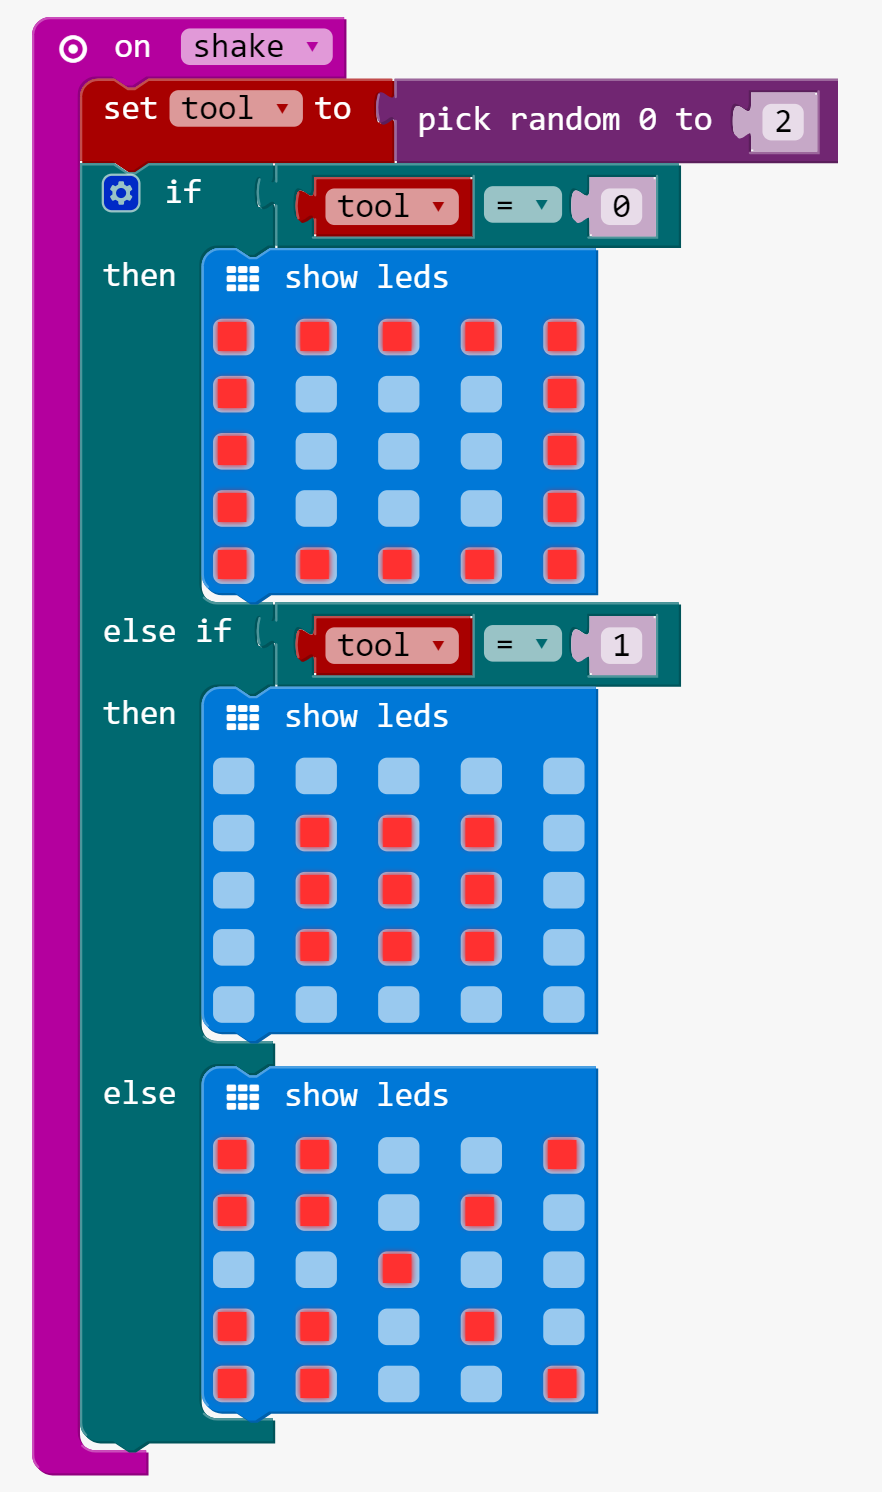
\includegraphics[width=1.5in]{images/rpsBlocks.png} \\
        (a) & (b) 
      \end{tabular}
    \caption{\label{fig:rps}Micro:bit watch for playing rock, paper, scissors game.}
\end{figure}

\subsection{Wear and Sense}

Figure~\ref{fig:rps} shows one of the most popular starting micro:bit projects:
a micro:bit watch that plays the rock-paper-scissors game; the program reacts
to a shake event by choosing a random number from the set \{0, 1, 2 \}
and displaying a rock, paper or scissor shape on the LED display. The
user can use this simple app to play the game by themselves or with
a friend. The project consists of a making step and coding step,
as shown at
\begin{center}
\url{https://makecode.microbit.org/projects/rock-paper-scissors}
\end{center}

% love meter
% - on pin pressed
% - display random number

% https://labs.redweb.com/project/controlling-music-with-movement/

\begin{figure} 
    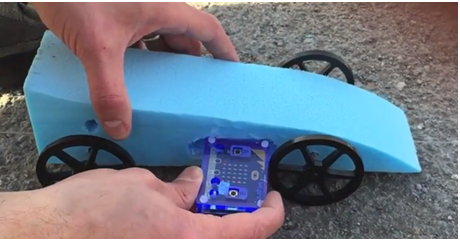
\includegraphics[width=3.3in]{images/rocketcar.png} 
    \caption{\label{fig:rocketcar}Bloodhound Model Rocket Car with embedded micro:bit for
    measuring acceleration.}
\end{figure}

\subsection{Measure}

The micro:bit's built-in sensors and small size make it perfect for embedding
in science and technology projects.  The Bloodhound Model Rocket Car is 
part of the Bloodhound Project,~\footnote{\url{www.bloodhoundssc.com}} 
whose goal is to set a new world land speed
record and inspire students about STEM subjects. 
Students design, build and race model rocket cars in competition, learning about
physics, aerodynamics, and mechanical engineering. Microsoft worked with
the Bloodhound Project to incorporate a micro:bit into the car's design,
as shown in Figure~\ref{fig:rocketcar};
the micro:bit captures the (X,Y,Z) accelerometer data of the rocket car
during its race. After the race, students can upload the data from 
the micro:bit and analyze the performance of their cars. 

% Bloodhound rocket car:
% - http://www.bloodhoundssc.com/news/launched-bbc-microbit-model-rocket-car-competition-%E2%80%9Crace-line%E2%80%9D
%

% https://makecode.microbit.org/projects/soil-moisture

\begin{figure} 
    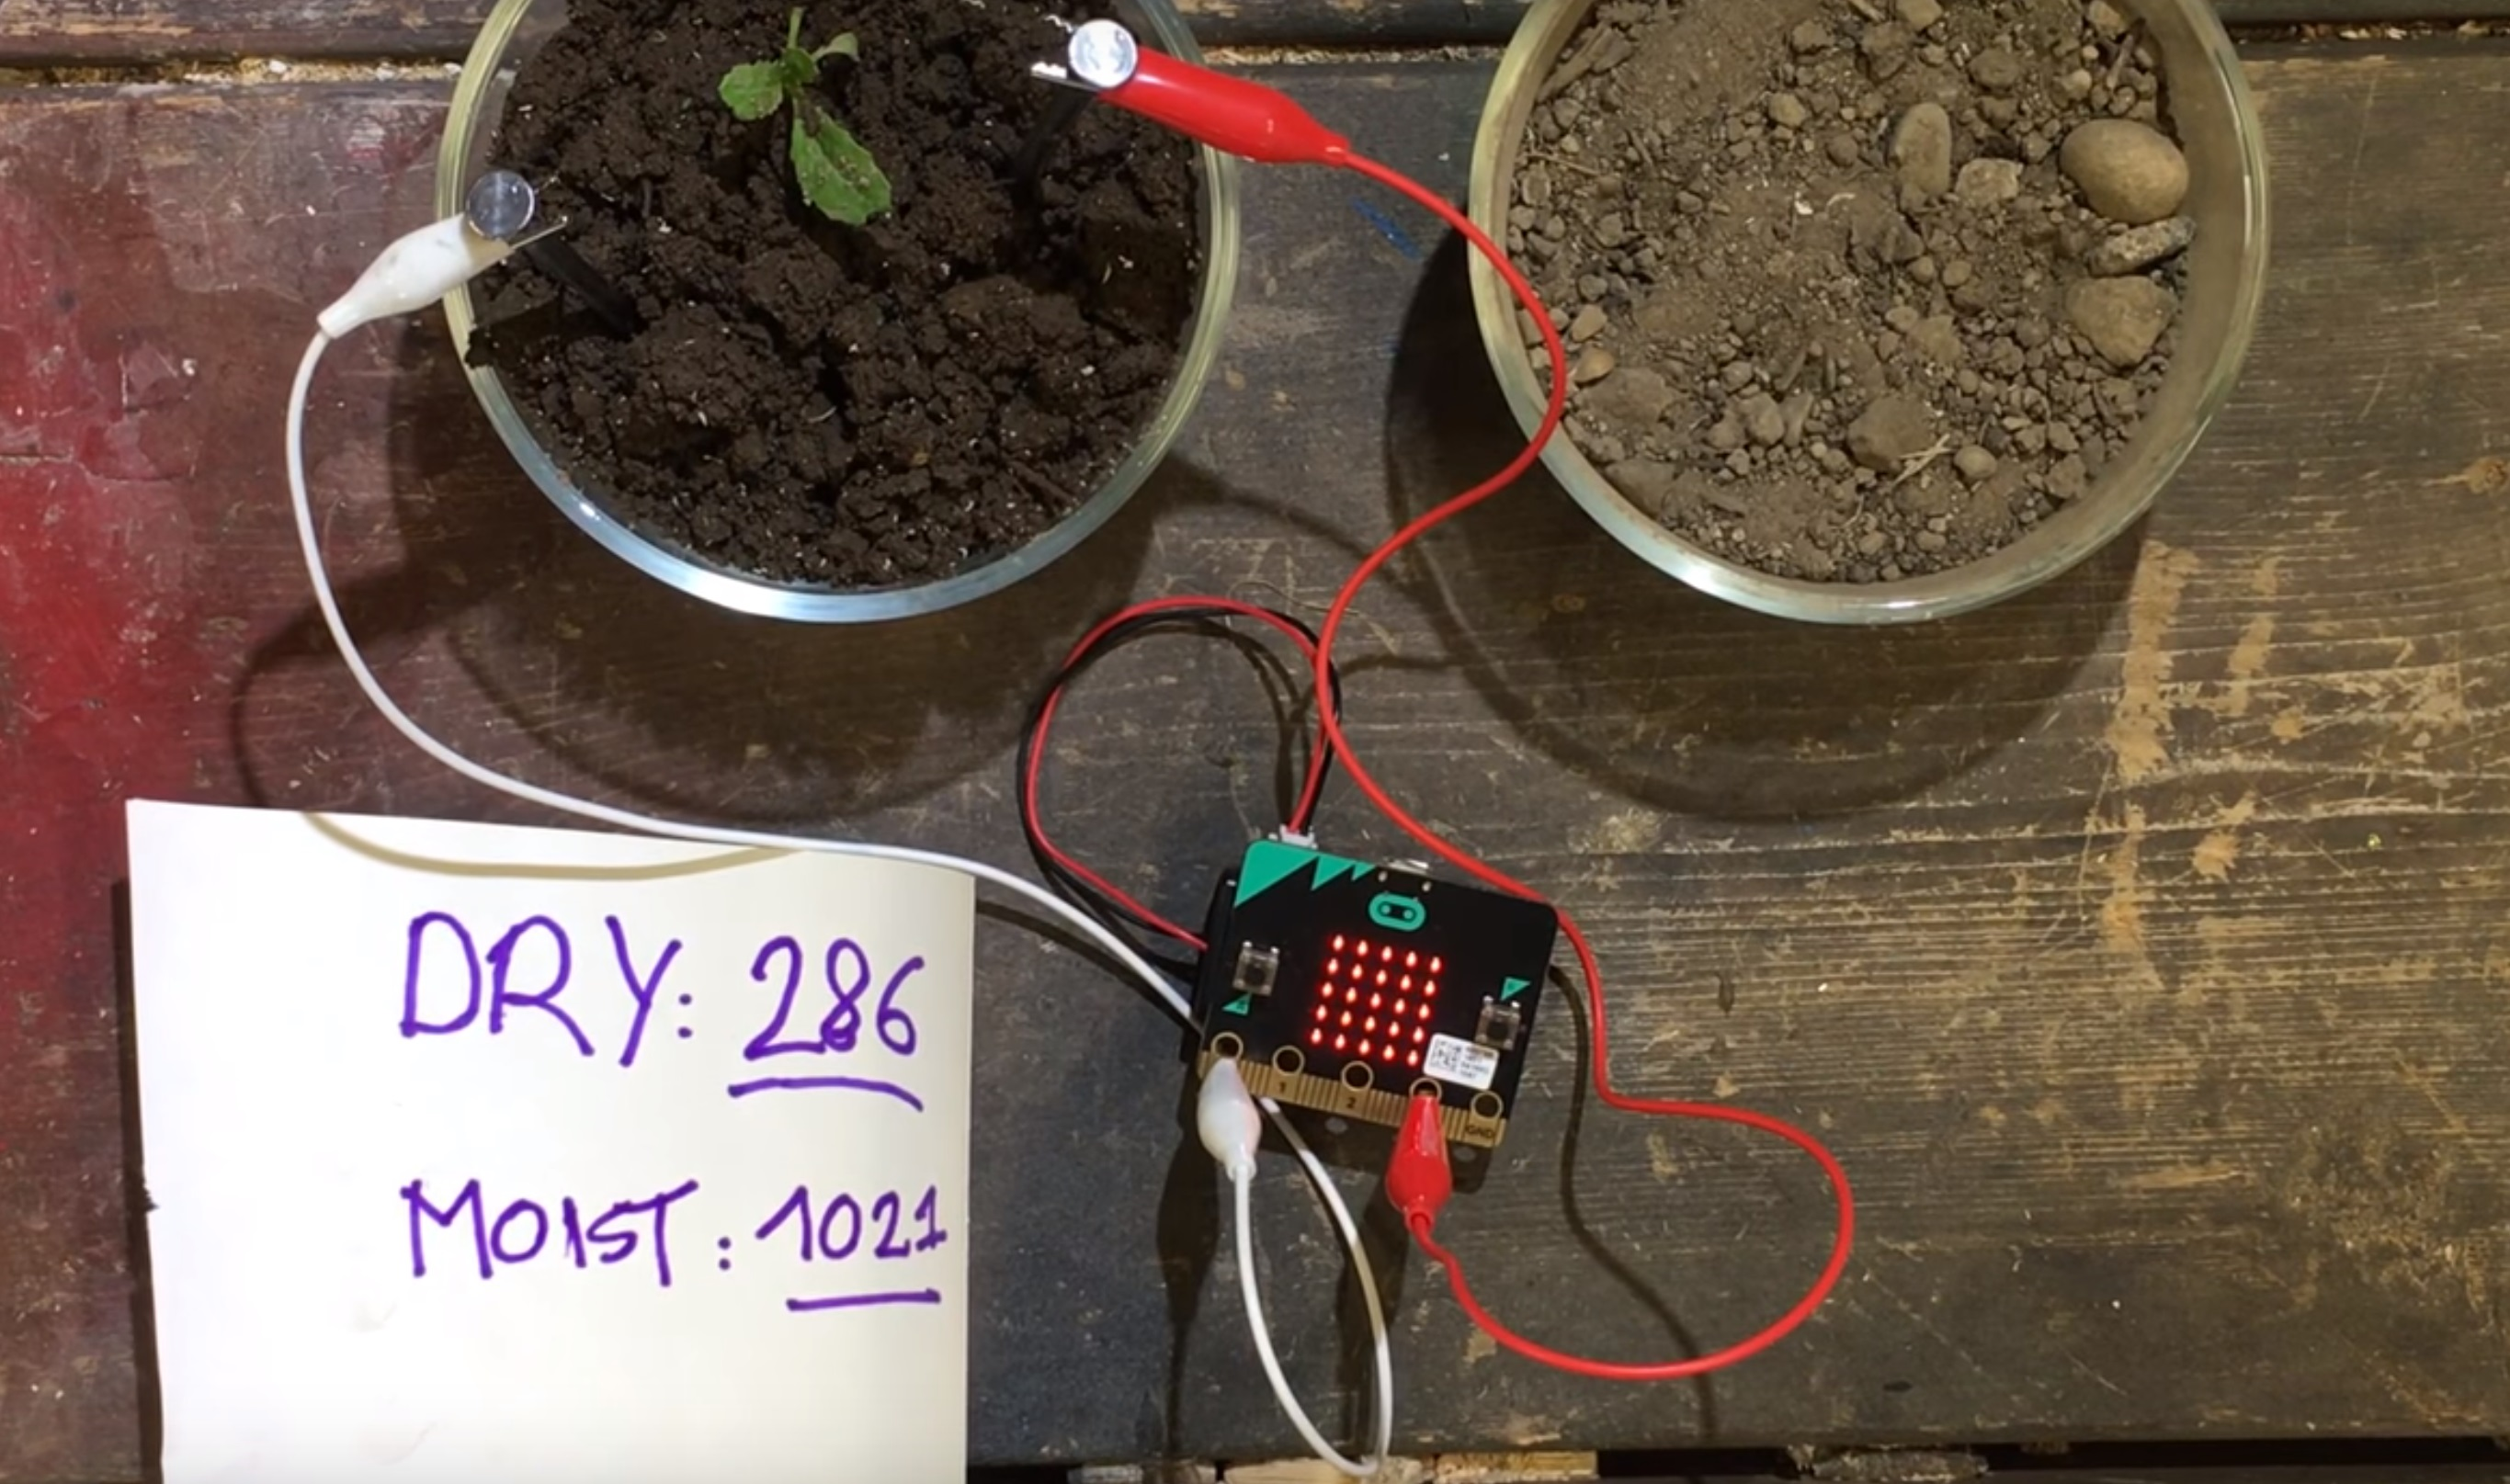
\includegraphics[width=3.3in]{images/moisture.png} 
    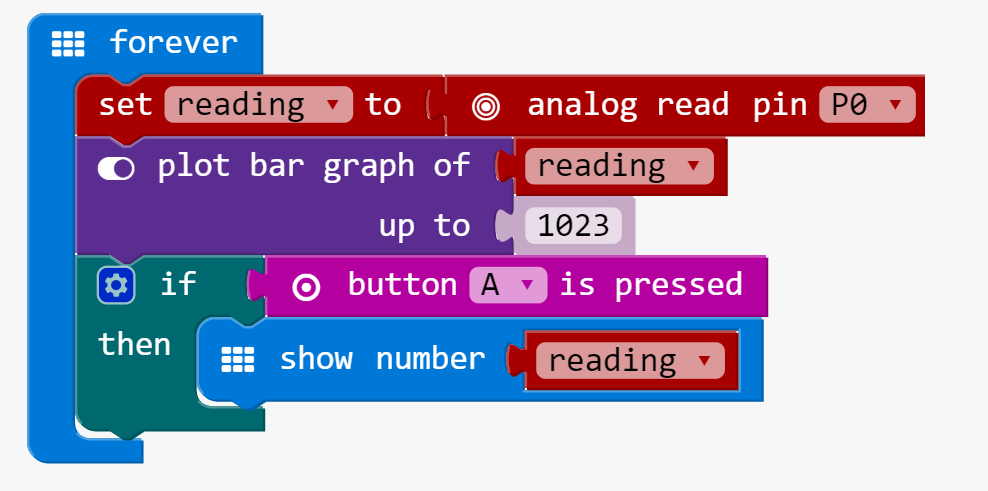
\includegraphics[width=3.3in]{images/moistureBlocks.png} 
    \caption{\label{fig:moisture}Measuring soil moisture via micro:bit pins.}
\end{figure}

Soil itself has some electrical resistance which depends on the amount of water 
and nutrients in it. It acts like a variable resistor in an electronic circuit. 
The water is not conductive but the nutrient content is. The combination of water 
and soil nutrients makes the soil have some conductivity. So, the more water there is, 
combined with the nutrients, the less the soil will have electrical resistance.


\subsection{Control}

% light sensor and servo
% https://makecode.microbit.org/projects/milk-carton-robot


% https://makecode.microbit.org/projects/soil-moisture

\subsection{Network}

% buttons, radio, display

% mood radio: https://makecode.microbit.org/projects/mood-radio
% voting: https://makecode.microbit.org/projects/voting-machine

% https://makecode.microbit.org/projects/fireflies
% https://makecode.microbit.org/projects/micro-coin

% - radio


